\chapter{Control approach in 2D space}\label{ch:controlapproach}

Control approach is based on previous theorem \ref{theorem1} and definitions  \ref{def:crashdistance}, \ref{ref:voting}, \ref{def:controlstrategy}. Control approach is switching control (fig. \ref{fig:ControlConcept}), between:
\begin{enumerate}[1.]
    \item\textit{Path following control} - system is following trajectory given by set of waypoints \\$\mathscr{W}_p = \left \{ w_1,w_2,\dots, w_n\right\}$, where $w_i = [x,y,z], i \in \left\{1,\dots,n\right\}$ is waypoint in global coordinate frame
    \item\textit{Emergency avoidance module} - executed when dangerous obstacles are detected in field of vision(FOV), which is defined in 2D by touple $[d_l,\theta_l]$, where $d_l$ is LiDAR range and $\theta_l$ is LiDAR effective detection angle.
\end{enumerate}


Control concept have been introduced and its displayed in fig. \ref{fig:ControlConcept}. For the sake of simplicity, control input of system (\ref{eq:uni1}, \ref{eq:uni2}, \ref{eq:uni1}) will be given by $\omega(t) = 0$ in \textit{Path following} mode and by (\ref{eq:avoidanceStrategy})  in \textit{Emergency avoidance} mode. Flight speed $v(t)$ will be equal to constant all time.

\section{Obstacle avoidance based on reach sets}\label{sec:obstacleavoidancetheorem}
Goal of future thesis is to formulate obstacle avoidance theorem based on reach set. Theorem will define constraints and conditions for reach set, where vehicle will never crash and to define control which allows weak invariance.

\begin{definition}{Obstacle $o \in \R^2$}\label{def:2dobst}
\\Vehicle in $\R^2$ space is characterized by its position $\vec{x} = [x_o, y_o]$ and heading $\theta$ \textit{Let} us define obstacle $o_i$: as vector with following properties: 
\begin{equation}
o_i = [x_o , y_o, \delta_o, \theta_o, \theta_b,d_o, d_c ]^t
\end{equation}
where:
\begin{enumerate}
    \item Obstacle position in local euclidean space as $[x_o, y_o]$.
    \item Obstacle angle $\theta_o \in (-\pi,\pi>$:
    \begin{equation}
        \theta_o = \textnormal{atan} (y_o - y_p,x_o - x_p)
    \end{equation}
    
    \item Obstacle heading angle $\theta_b$:
    \begin{equation}\label{eq:obstacleHeadingAngle}
        \theta_b = \theta_o - \theta
    \end{equation}
    
    \item Distance to obstacle $d_o$ as euclidean norm:
    \begin{equation}
        d_o = \lVert [x_o y_o] - \vec{x} \rVert_{\xi}
    \end{equation}
    
    \item Crash distance $d_c$:
    \begin{equation}\label{eq:crashdistance}
        d_c = f(d_o,\theta_b);
    \end{equation}
    
    \item Danger level $\delta_o$ defined by following function:
    \begin{equation}
    \delta_o =
    \begin{cases}
        1 & d_c \leq d_o \wedge |\theta_b| \le \frac{\pi}{2}\\
        2 & d_c \leq d_o \wedge |\theta_b| > \frac{\pi}{2}\\
        0 & \textnormal{otherwise}
    \end{cases}
    \end{equation}
\end{enumerate}
\end{definition}

\begin{note}{Danger level $\delta_o$}
    \\One can say, danger level is $\delta_o = 0$ when obstacle is far away from plane, class of obstacle is $\delta_o = 1$ when obstacle is near and in front of plane local position(\textit{Crash constraint}), class of obstacle is $\delta_o = 2$ when obstacle is near and in back of plane (\textit{Turn constraint}).
\end{note}


\begin{definition}{Threat set $\mathscr{D}$}\label{def:threatset}
Then threat set $\mathscr{D}$,  represents threading obstacles which are limiting plane turning or will be crashed into obstacle.
\begin{equation}
\mathscr{D} = \{\forall o_i: \delta_{oi} \in \{1,2\}\} 
\end{equation}
\end{definition}

\begin{theorem} {Unicycle obstacle avoidance}\label{theorem1}
\\For given system of unicycle (\ref{eq:uni1}, \ref{eq:uni2}, \ref{eq:uni3}),with state (\ref{eq:uni4}), and input (\ref{eq:uni5}) with constant speed of vehicle $v = 1 m/s$.\\
\\
\textit{Let} us define control input function $ \omega(\vec{x},\mathscr{O}) \in \Omega$ where control strategy $\Omega$ is defined as follow:
\begin{equation}
\label{eq:omegaswitch}
\omega(\vec{x},\mathscr{O}) =
    \begin{cases} 
      -\frac{\pi}{12} & \textnormal{turn right}\\
      0 & \textnormal{fly straight} \\
      \frac{\pi}{12}  & \textnormal{turn left} 
   \end{cases}
\end{equation}
Obstacle set $\mathscr{O}$ in known world, defined as follow:
\begin{equation}
    \mathscr{O} = \{\forall o_i: o_i \in \textnormal{sensor range}  \vee \textnormal{buffer}\}
\end{equation}
Each member value of obstacle $o_i$ is defined by (Def. \ref{def:2dobst}).
\\\\
\textit{There} exist minimal obstacle distance $\delta_s$, that unicycle reach set $R[\tau, t_0, \vec{x}_0]$, $\tau \in [t_0, \infty)$ will not contain any obstacles $\vec{x_o} =[x_o, y_o]$.
\begin{equation}
    \label{eq:deltaw}
    \forall o_i \in \mathscr{O}, \lVert \vec{x}_0 - [x_{oi}, y_{oi}, \theta_{oi}]^T \rVert \ge \delta_s
\end{equation}
\end{theorem}



\newpage
\begin{dokaz}{Theorem \ref{theorem1}.}
\\Heading angle $\theta$ is determined by function  $\omega(\vec{x},\mathscr{O})$, by following expression:
\begin{equation}
    \theta(t) = \int_{t_0}^{t} \omega(\vec{x}(\tau),\mathscr{O}) d\tau + \theta(t_0)
\end{equation}
\\Position of vehicle is given by following expression:
\begin{equation}
    x(t) = \int_{t_0}^{t} v\cos\theta(\tau) d\tau + x(t_0)
\end{equation}
\begin{equation}
    y(t) = \int_{t_0}^{t} v\sin\theta(\tau) d\tau + y(t_0)
\end{equation}
\\Modified reach set $R[\tau, t_0, \vec{x}_0]$ from definition \ref{def:reachset01}:
\begin{equation}\label{eq:theoremset1}
    R[\tau, t_0, \vec{x}_0] = \bigcup \{[{x}(\tau),y(\tau)]^T,\theta(s),s \in (t_0,\tau]\}=
    \left \{
    \begin{bmatrix}
    x_r\\
    y_r
    \end{bmatrix}
    \right\}
    = \left \{ \vec{x}_r \right\}
    = \mathscr{R}
\end{equation}

Now show that $\mathscr{R} \cap \mathscr{O} = \emptyset$, lets coat every obstacle $o_i \in \mathscr{O}$ with circle set defined by border $(x - x_{oi})^2 + (y-y_{oi})^2 = {d_{ci}}^2$, where $d_{ci}$ is obstacle crash distance given by crash distance function. Example of crash distance function (\ref{eq:crashdistance}) can be found in chapter \ref{sec:smartinvariance}. 
\\
\textit{Safety margin} should guarantee vehicle reaction to any detected obstacle. Obstacles are usually evaluated in some time period $t_s$ and with given vehicle velocity $v$, safety margin $s_m$ can be defined as:
\begin{equation}\label{eq:safetymargin}
    s_m = a.t_s.v;a \in <1,\infty) 
\end{equation}
\\
Finally define control strategy $\Omega(\vec{x}(t),\mathscr{O})$, with voting algorithm $\gamma(\mathscr{O})=\left\{-1,1\right\}$ as follow:
\begin{equation}\label{eq:avoidanceStrategy}
    \Omega(\vec{x}(t),\mathscr{O}) = 
    \begin{cases}
        \exists o_i \in \mathscr{O}: d_{oi} \le (d_{ci} + s_m) & : \omega(\vec{x}(t),\mathscr{O})=\gamma(\mathscr{O})\frac{\pi}{12}\\
        \exists! o_i \in \mathscr{O}: d_{oi} \le (d_{ci} + s_m)c & : \omega(\vec{x}(t),\mathscr{O}) \in \left\{\ -\frac{\pi}{12},0,\frac{\pi}{12} \right\}
    \end{cases}
\end{equation}
\\
Equation (\ref{eq:avoidanceStrategy}) can be interpreted as follow, if there exist dangerous obstacle $oi$, where distance to obstacle $d_o$ is lesser than crash distance $d_c$ with added safety margin $s_m$, then control strategy $\Omega$ limits possible control input to $\omega = \gamma(\mathscr{O})\frac{\pi}{12}$. Control input $\omega$ can be described as \textit{sharp turn right} or \textit{sharp turn left}, based on voting algorithm $\gamma(\mathscr{O})$.
\\\\
By proposing crash distance function (\ref{eq:crashdistance}) and safety margin (\ref{eq:safetymargin}) with minimal obstacle distance $\delta_s$, given by inequality:
\begin{equation}
    \delta_s \ge s_m + \sup{\left\{d_c:d_c \in o_i, o_i \in \mathscr{O}, \ \textnormal{at}\  t_0\right\}}
\end{equation}
\\Any starting point $\vec{x}(t_0)$ which satisfies (\ref{eq:deltaw}), reach set $\mathscr{R}$ defined by (\ref{eq:theoremset1}) can not reach any obstacle $o_i \in \mathscr{O}$.
Therefore $\mathscr{R} \cap \mathscr{O} = \emptyset$ and theorem \ref{theorem1}. is proven
\end{dokaz}

\subsection{Practical implications}
Previous theorem has throw up some definitions of partial functions. Given avoidance principle for unicycle is giving a theoretical framework of functions, these functions can be later used in general avoidance theorem formulation. Other practical implication is usage of these definitions in control design in chapter \ref{ch:controlapproach}. Practical implications of presented theorem can be summarized in following definitions:

\begin{definition}{Crash distance function $f$}\label{def:crashdistance}
\\For every obstacle $o \in \mathscr{O}$ there exist evaluation function $f(o,\vec{x}(t),\mathscr{O})$ which assess crash distance $d_c$ as a property of obstacle $o$. Crash distance $d_c$ is dynamic property depending on:
\begin{enumerate}
    \item $[x_v,y_v,z_v]$ vehicle position ($\vec{x}(t)$).
    \item $[\phi_v,\theta_v,\psi_v]$ vehicle orientation ($\vec{x}(t)$).
    \item $v_v$ vehicle speed ($\vec{x}(t)$).
    \item $[x_o,y_o,z_o]$ obstacle position ($o_i \in \mathscr{O}$).
    \item $[\phi_o,\theta_o,\psi_o]$ obstacle orientation ($o_i \in \mathscr{O}$).
    \item $v_o$ obstacle speed ($o_i \in \mathscr{O}$).
\end{enumerate}
Obstacle distance function $f(o,\vec{x}(t),\mathscr{O})$ can be viewed as standard threat assessment function from viewpoint of game theory.
\end{definition}

\begin{definition}{Voting algorithm $\gamma$}\label{ref:voting}
\\Let $\mathscr{U}$ be set of available control strategies $u(t)$ for system $\dot{x}=f(t,x,u)$. Known dangers are accumulated in set $\mathscr{D}$, in general formulation known obstacle set $\mathscr{O}$ is used. Each obstacle $o_i$ have property $d_i$ and other threat properties assessed. Then optimal control strategy $u(t) \mathscr{U}$ is chosen by voting algorithm $\gamma(\vec{x}(t),\mathscr{U},\mathscr{O})$, where $\vec{x}(t)$ is state of vehicle including position, orientation and movement speed. 
\begin{equation}
   u(t)= \gamma(\vec{x}(t),\mathscr{U},\mathscr{O})
\end{equation}
Note: set $\mathscr{U}$  is defined by control strategy defined by \ref{def:controlstrategy}.
\end{definition}

\begin{definition}{Control strategy $\Omega$}\label{def:controlstrategy}
\\Control strategy $\Omega:\R^n\times\mathscr{O}\to\left\{\R^k\right\}$ is function which outputs possible control moves set $u(t) \in \mathscr{U}$, $\mathscr{U}$ can be defined as:
\begin{enumerate}
    \item \textit{Continuous signals} -  set of safe continuous inputs.
    \\$\mathscr{U} = \left \{ u_1(t),u_2(t),\dots,u_n(t)\right\}$
    \item \textit{Discrete signals} - set of safe discrete inputs, defined for decision time $t_S$.
    \\$\mathscr{U} =  \left\{ u_1(\tau,\tau+t_s),u_2(\tau,\tau+t_s),\dots,u_n(\tau,\tau+t_s)\right\}$
    \item \textit{Continuous signal sequences} - set of continuous/discrete signal sequences, switching time between signals in subset is determined by control on later stages.
    \\$\mathscr{U} = \left\{\left\{u_{11}(t),u_{12}(t),\dots,u_{1n}(t)\right\},\dots,\left\{u_{m1}(t),u_{m2}(t),\dots,u_{mn}(t)\right\}\right\}$
\end{enumerate}
\end{definition}

\begin{note}
    Example of control strategy and voting algorithm can be seen at (\ref{eq:avoidanceStrategy})
\end{note}


\section{Emergency avoidance module}\label{s:emergencyAvoidanceModule2D}
Emergency avoidance module is running in safe time intervals $t_s =1s$, space representation of FOV is divined into cells determined by \textit{distance interval}: $0:\delta_d:d_l$ and \textit{angle interval}: $0:\delta_\theta:\theta_l$, where $\delta_d$ is length step and $\delta_\theta$ is angle step respectively. FOV $\mathscr{F}$ is represented as set of cells $\mathscr{C}_i \in \mathscr{F}$ with borders for distance span and angle span:
\begin{equation}\label{eq:FOVrepresentation}
    \mathscr{F}=\left\{
    \begin{bmatrix}
    0 & \delta_d\\
    0 & \delta\theta
    \end{bmatrix},
    \begin{bmatrix}
    \delta_d & 2\delta_d\\
    \delta\theta & 2\delta\theta
    \end{bmatrix},\dots
    \begin{bmatrix}
    (n-1)\delta_d & n\delta_d\\
    (n-1)\delta\theta & n\delta\theta
    \end{bmatrix}
    \right\}
    = \left\{\mathscr{C}_0,\mathscr{C}_1,\dots\mathscr{C}_n\right\}
\end{equation}
Representation (\ref{eq:FOVrepresentation}) can be easily extended to third dimension by defining \textit{horizontal plane angle} $\theta$ and \textit{vertical plane angle} $\varphi$.
Emergency avoidance module in this case consist of following algorithms:
\begin{enumerate}
    \item \textit{Obstacle detection} (fig. \ref{fig:ObstacleDetection}) - detect obstacles in known space.
    \item \textit{Uncertainty assessment} (fig. \ref{fig:UncertaintyAssesment}) - assess uncertain areas which are in known space, but they are hidden behind detected obstacles.
    \item \textit{Reachable space assessment} (fig. \ref{fig:ReachableSpace}) - calculate reachable space in free known space.
    \item \textit{Avoidance execution} (fig. \ref{fig:PathCalculation}) - calculate avoidance strategy $\Omega$ and consider avoidance execution by voting algorithm $\gamma$.
\end{enumerate}
Because avoidance algorithm is running in periodical time $t_s$, plane needs to have a space to turn in case of blocked path, therefore FOV $\mathscr{F}$ is divined into following areas (fig. \ref{fig:FieldOfViewZones}):
\begin{enumerate}
    \item\textit{Safe area} - area where vehicle have place to turn back in case there does not exist path to avoid end of \textit{Avoidance area}.
    \item\textit{Avoidance area} - area where vehicle suppose to execute avoidance maneuvers given by control strategy $\Omega$ and voting algorithm $\gamma$.
    \item\textit{Crash area} - area which is uncertain and can cause vehicle crash.
\end{enumerate}

\begin{figure}[H]
    \begin{subfigure}{0.5\textwidth}
    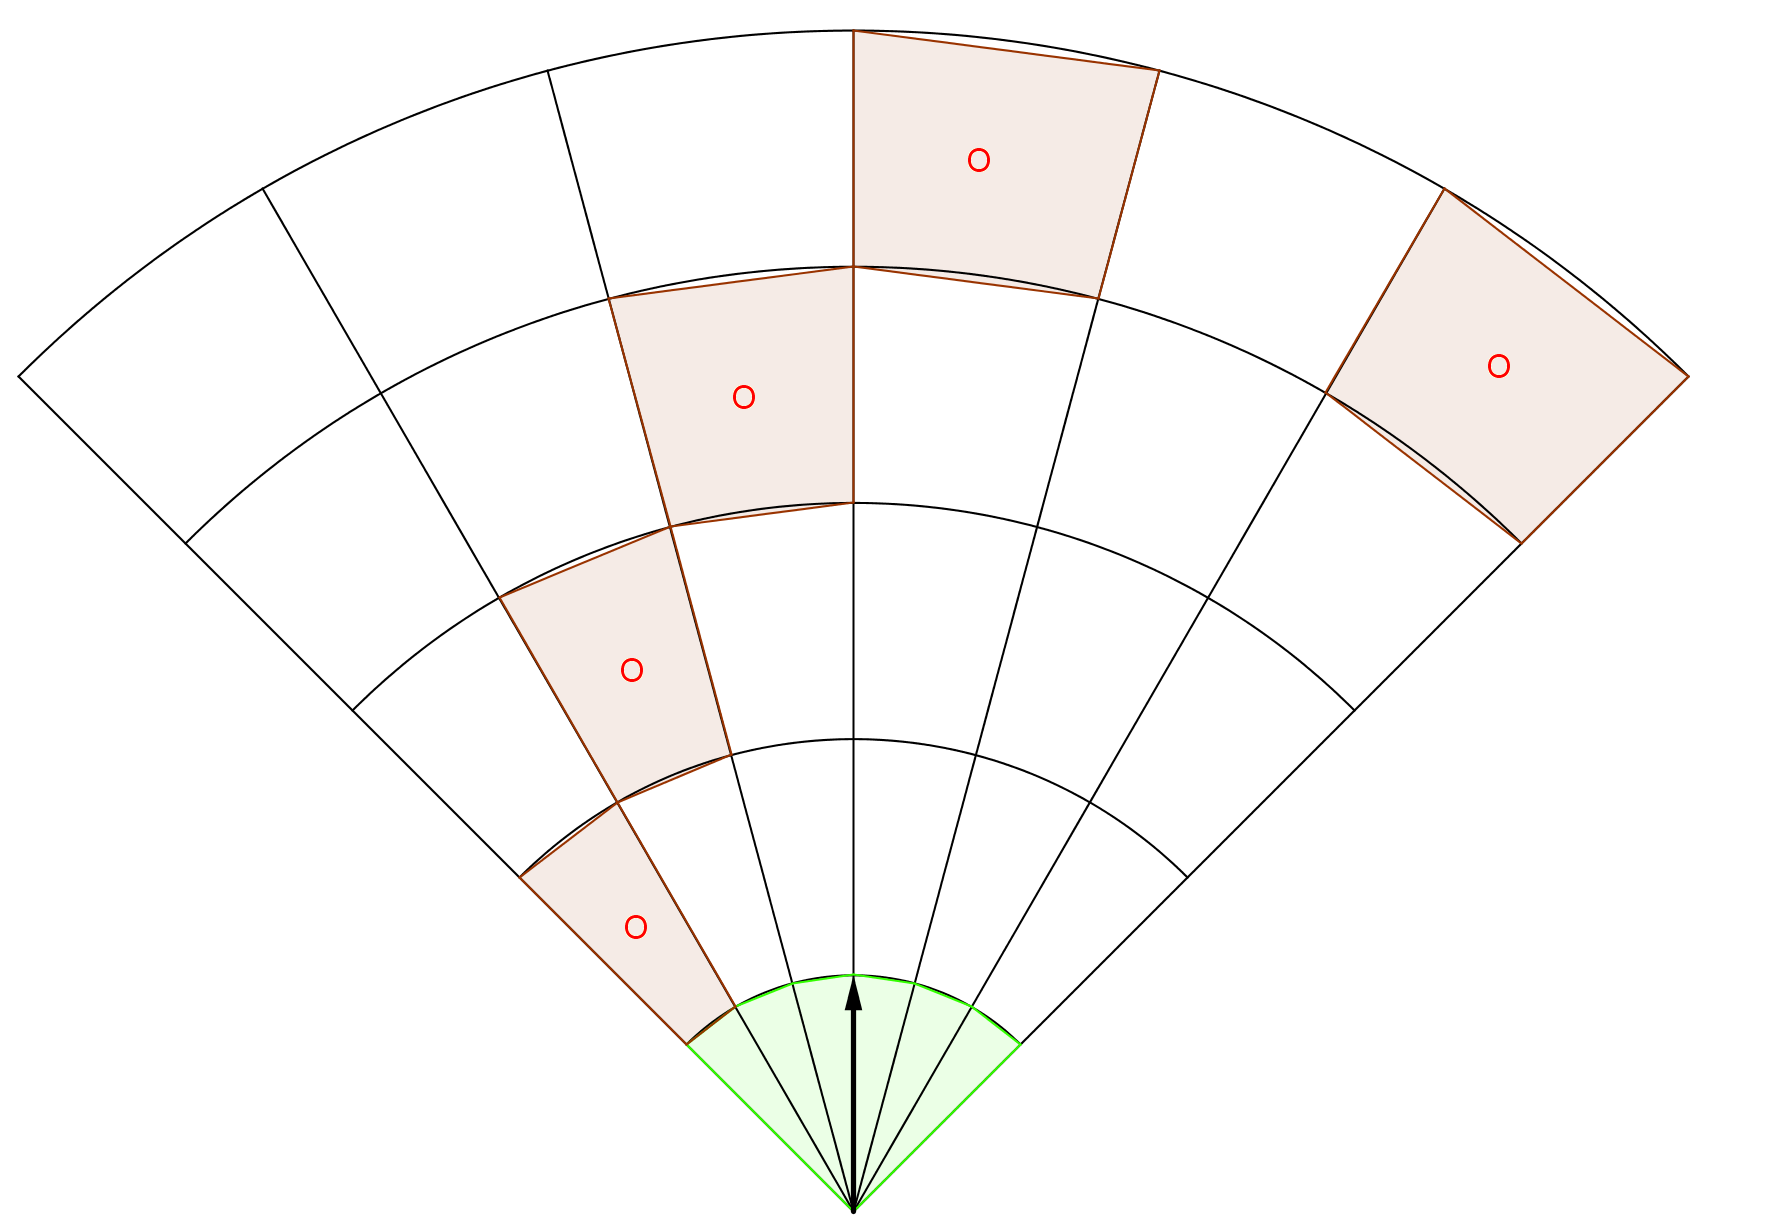
\includegraphics[width=0.9\linewidth]{\FIGDIR/04ObstacleDetection.png} 
    \caption{Obstacle detection}
    \label{fig:ObstacleDetection}
    \end{subfigure}
    \begin{subfigure}{0.5\textwidth}
    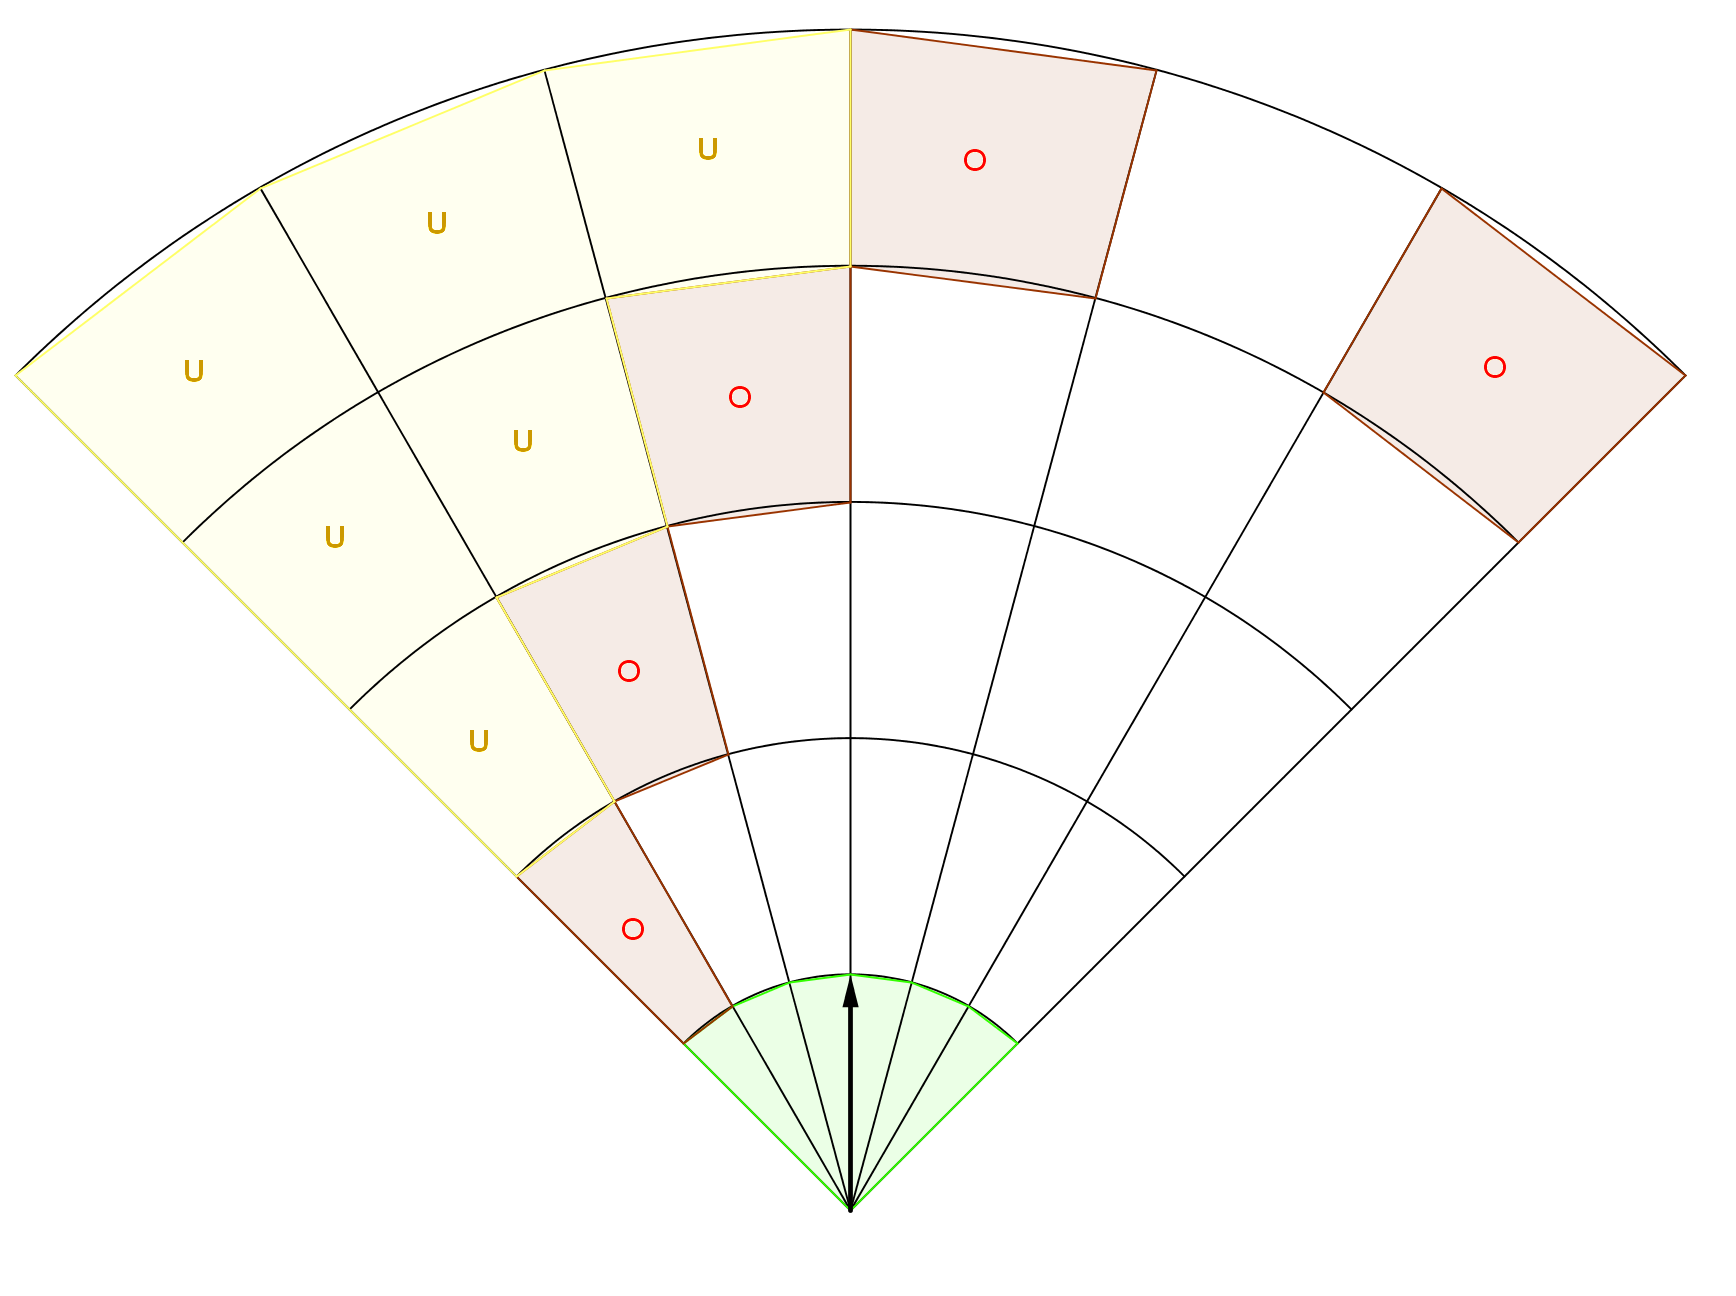
\includegraphics[width=0.9\linewidth]{\FIGDIR/05UncertainityAssesment.png}
    \caption{Uncertainty assessment}
    \label{fig:UncertaintyAssesment}
    \end{subfigure}
\caption{Determination of accessible space}
\label{fig:AccessibleSpace}
\end{figure}


Building of known space $\mathscr{F}$ and known obstacles $\mathscr{O}$ (\ref{fig:AccessibleSpace}) is based on LiDAR detection range $\mathscr{F}_D$ (\ref{eq:FOVrepresentation}). This particular space is divided into following sets: \textit{obstacle set} $\mathscr{O}_D$, \textit{uncertain set} $\mathscr{O}_U$, and \textit{free set} $\mathscr{O}_F$. Vehicle position is in known space $\mathscr{F}$, free space in known space is given as $\mathscr{F}-\mathscr{O}$. Reachable space $\mathscr{R}$ is not equal to free space. Known space $\mathscr{F}$ and known obstacles $\mathscr{O}$ are updating as follow: 

\begin{algorithm}[H]
 $\mathscr{F}_D=\{$FOV$\}$\;
 $\mathscr{O}_D = \{\mathscr{C}\in\mathscr{F_D}$; where obstacle is detected$\}$ \;
 $\mathscr{O}_U = \{\mathscr{C}\in\mathscr{F_D}$; where FOV is obscured by $ \mathscr{O}_D\}$ \;
 $\mathscr{O}_F = \{\mathscr{C}\in\mathscr{F_D}$; where is free space inside FOV $\}$ \;
 \eIf{$\mathscr{O}$ exist}{
    $\mathscr{O}=\mathscr{O}\cup\mathscr{O}_D\cup\mathscr{O}_U-\mathscr{O}_F$}{
    $\mathscr{O}= \mathscr{O}_D\cup\mathscr{O}_U$}
 \eIf{$\mathscr{F}$ exists}{
 $\mathscr{F} = \mathscr{F}\cup\mathscr{F}_D$}{
 $\mathscr{F} = \mathscr{F}_D$}
 \caption{Accessible space assessment}
\end{algorithm}

Building reachable space $\mathscr{R} \in (\mathscr{F} - \mathscr{O})$ its incremental process. First goal $\mathscr{G} \in \mathscr{F}$ is determined, goal can be:
\begin{enumerate}
    \item\textit{Follow up waypoint $w_i$} - waypoint in alignment of $\mathscr{W}$ if there exist free path in known world $\mathscr{F}$.
    \item\textit{Return waypoint $w_r$} - waypoint leading to undiscovered area close to path given by $\mathscr{W}$ in known world $\mathscr{F}$ in case known obstacles $\mathscr{O}$ are forming trap in known world $\mathscr{F}$.
\end{enumerate}

\begin{figure}[H]
    \begin{subfigure}{0.5\textwidth}
    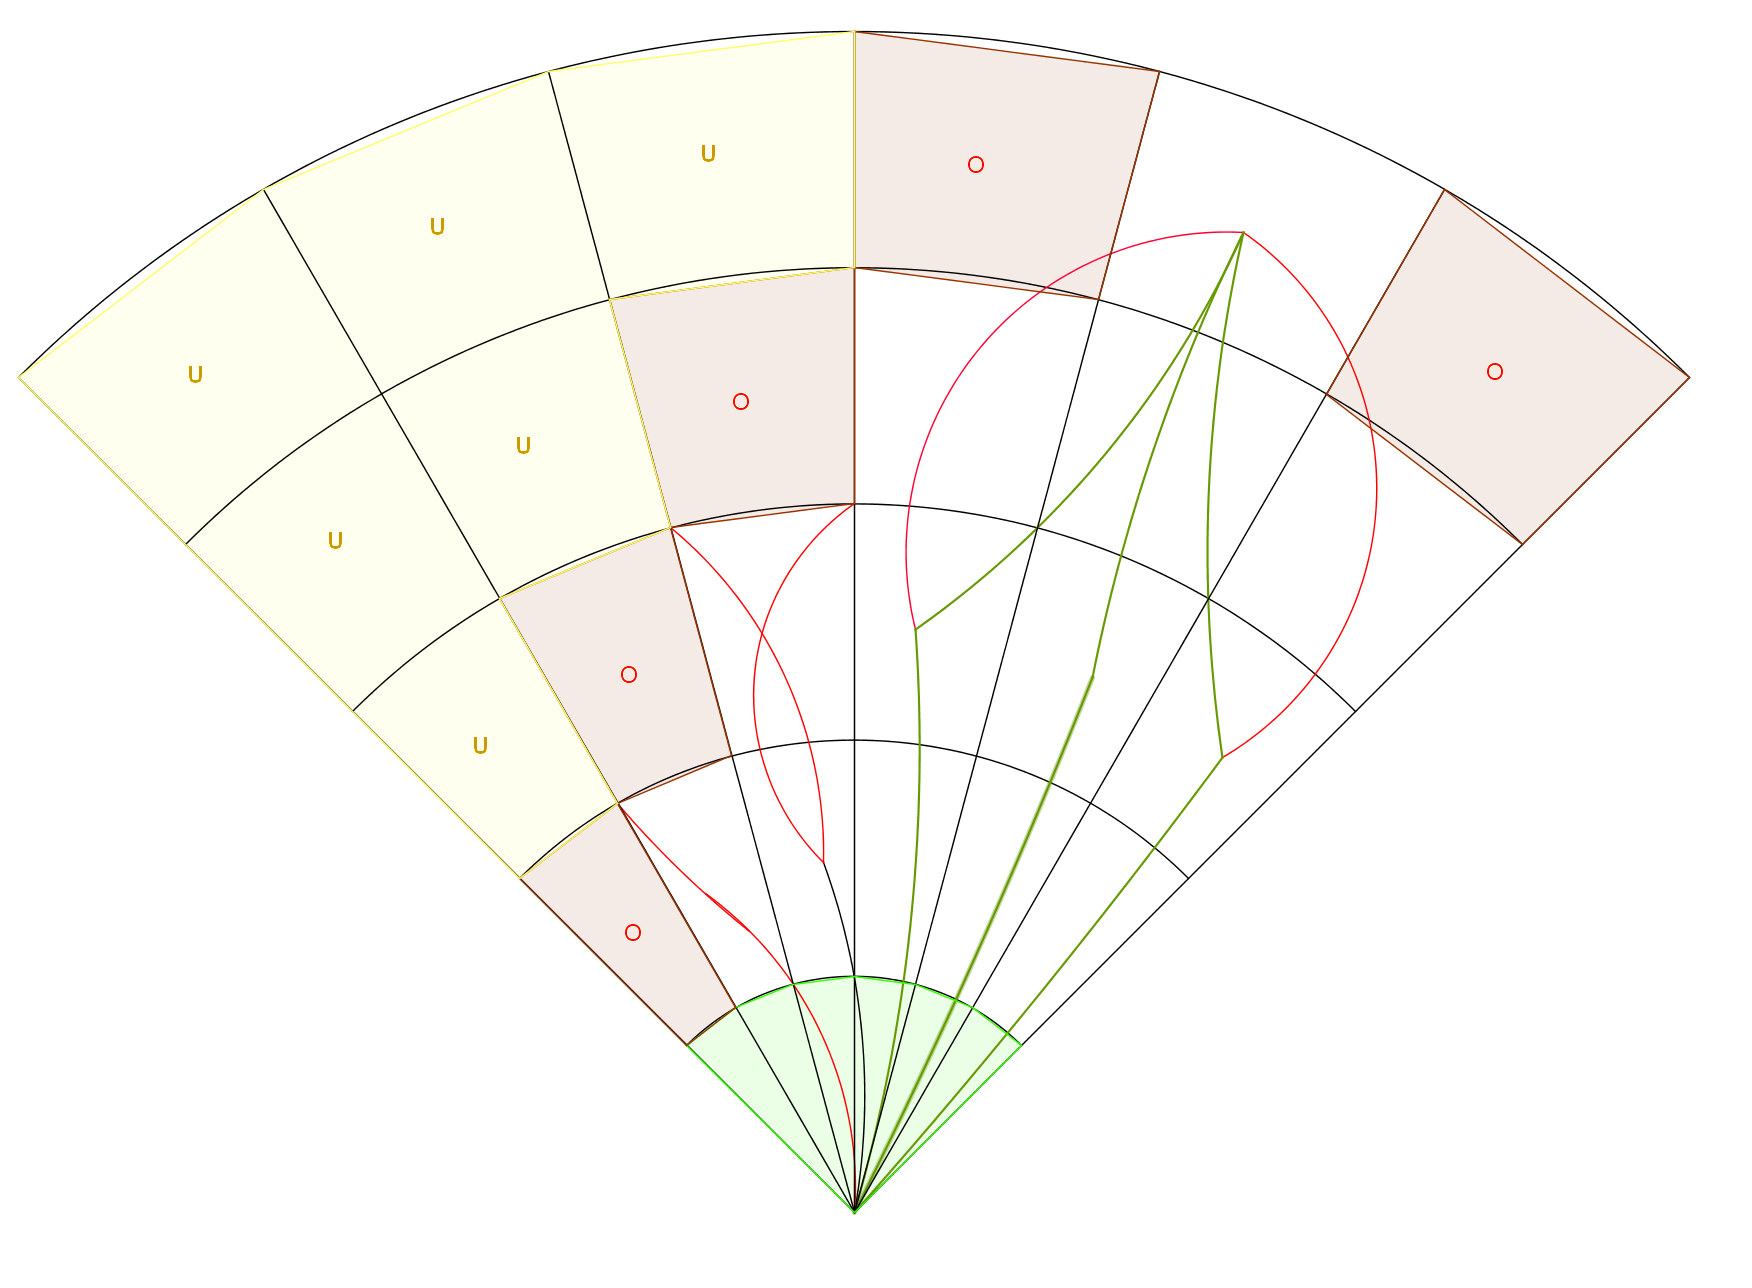
\includegraphics[width=0.9\linewidth]{\FIGDIR/06SurveyOfVacantSpace.png} 
    \caption{Survey of vacant space}
    \label{fig:SurveyOfVacantSpace}
    \end{subfigure}
    \begin{subfigure}{0.5\textwidth}
    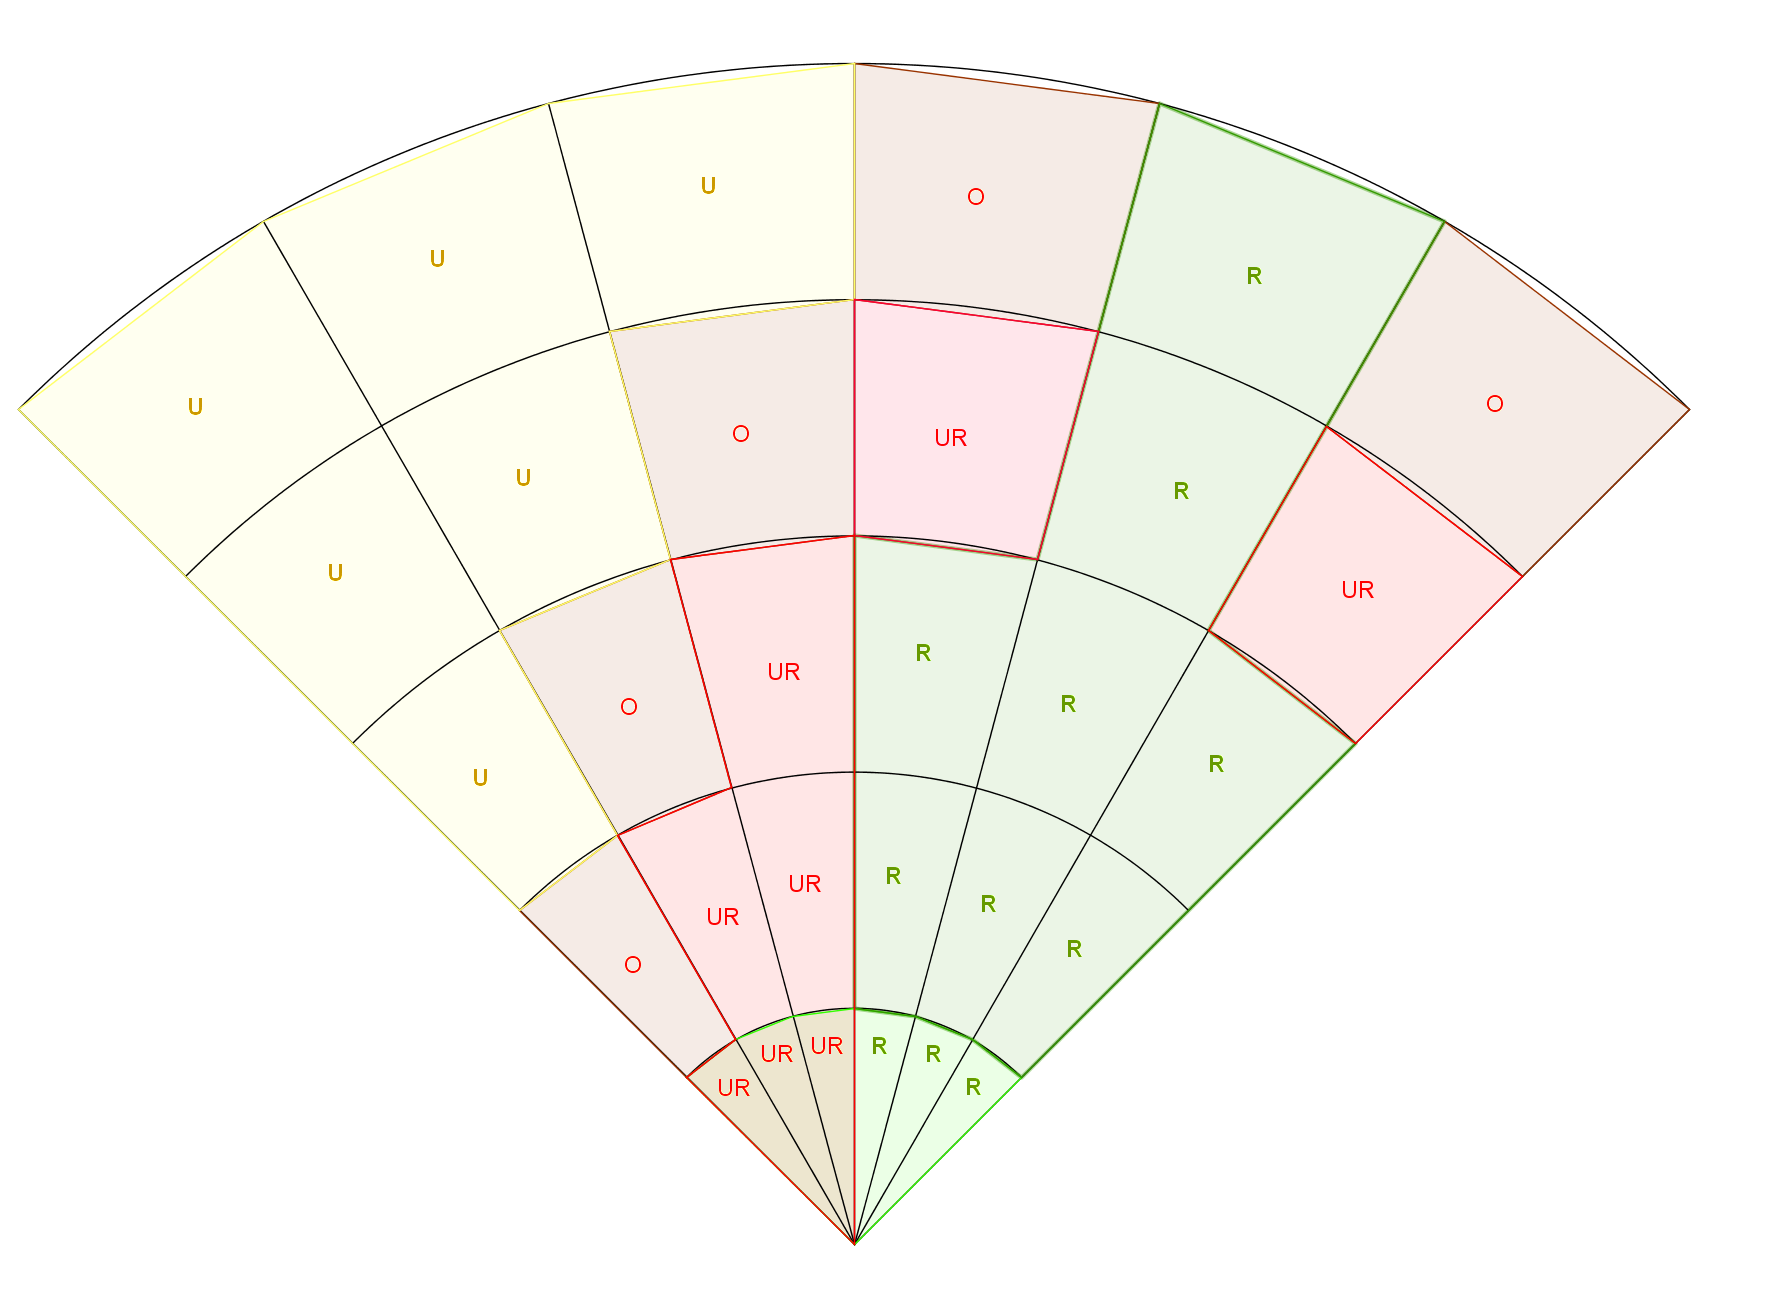
\includegraphics[width=0.9\linewidth]{\FIGDIR/07ReachableSpaceAssesment.png}
    \caption{Reachable space assessment}
    \label{fig:ReachableSpaceAssesment}
    \end{subfigure}
\caption{Determination of reachable space}
\label{fig:ReachableSpace}
\end{figure}
Algorithm to determine reachable space operates in known world $\mathscr{F}$, where uncertain space $\bar{\mathscr{U}}$ and obstacle space $\bar{\mathscr{O}}$ are considered as merged obstacle space $\mathscr{O}=\bar{\mathscr{O}}\cup\bar{\mathscr{U}}$. Start point $\mathscr{S}$ is determined from vehicle state $\vec{x}$ or its future approximation. Reachable space $\mathscr{R}$ is in principle calculated by algorithm \ref{alg:reachablespace}., but reachable space estimation and calculation is main topic of future thesis. Therefore functions $buildTrajectory(x,\Omega,t_s)$ and $coatTrajectory(t)$ remains undefined at this moment.

\begin{algorithm}[H]
Determine $\mathscr{S}$ as start point from $\vec{x}$ vehicle state\;
Search space $\mathscr{E} = \mathscr{F}-\mathscr{O}$\;
Reachable space $\mathscr{R} =\emptyset$\;
Unreachable space $\mathscr{U}=\emptyset$\;
\For{$\vec{u}\in\Omega(\vec{x},\mathscr{O})$}{
    $\vec{x}=\mathscr{S}$\;
    $t=buildTrajectory(x,\Omega,t_s)$\;
    $T=coatTrajectory(t)$\;
    \eIf{$T\cap\mathscr{O}==\emptyset$}{
    $\mathscr{R}=\mathscr{R}\cup T$\;}{
    $\mathscr{U}=\mathscr{U}\cup T$\;}
}
\If{$(\mathscr{S}-(\mathscr{R}\cup\mathscr{U}))!=\emptyset$}{
$\mathscr{U}=\mathscr{U}\cup(\mathscr{S}-(\mathscr{R}\cup\mathscr{U}))$}
\caption{Reachable and unreachable space assessment}
\label{alg:reachablespace}
\end{algorithm}

Goal of avoidance maneuver $\mathscr{S}$ is calculated based on reachable set $\mathscr{R}$ and other criterion's. Avoidance trajectory is calculated based on available control strategy $\Omega$, start point $\mathscr{S}$, end point $\mathscr{G}$ and voting algorithm $\gamma$. Example of avoidance path in reachable space can be seen at (fig. \ref{fig:PathCalculation}).

\begin{figure}[H]
 
    \begin{subfigure}{0.5\textwidth}
    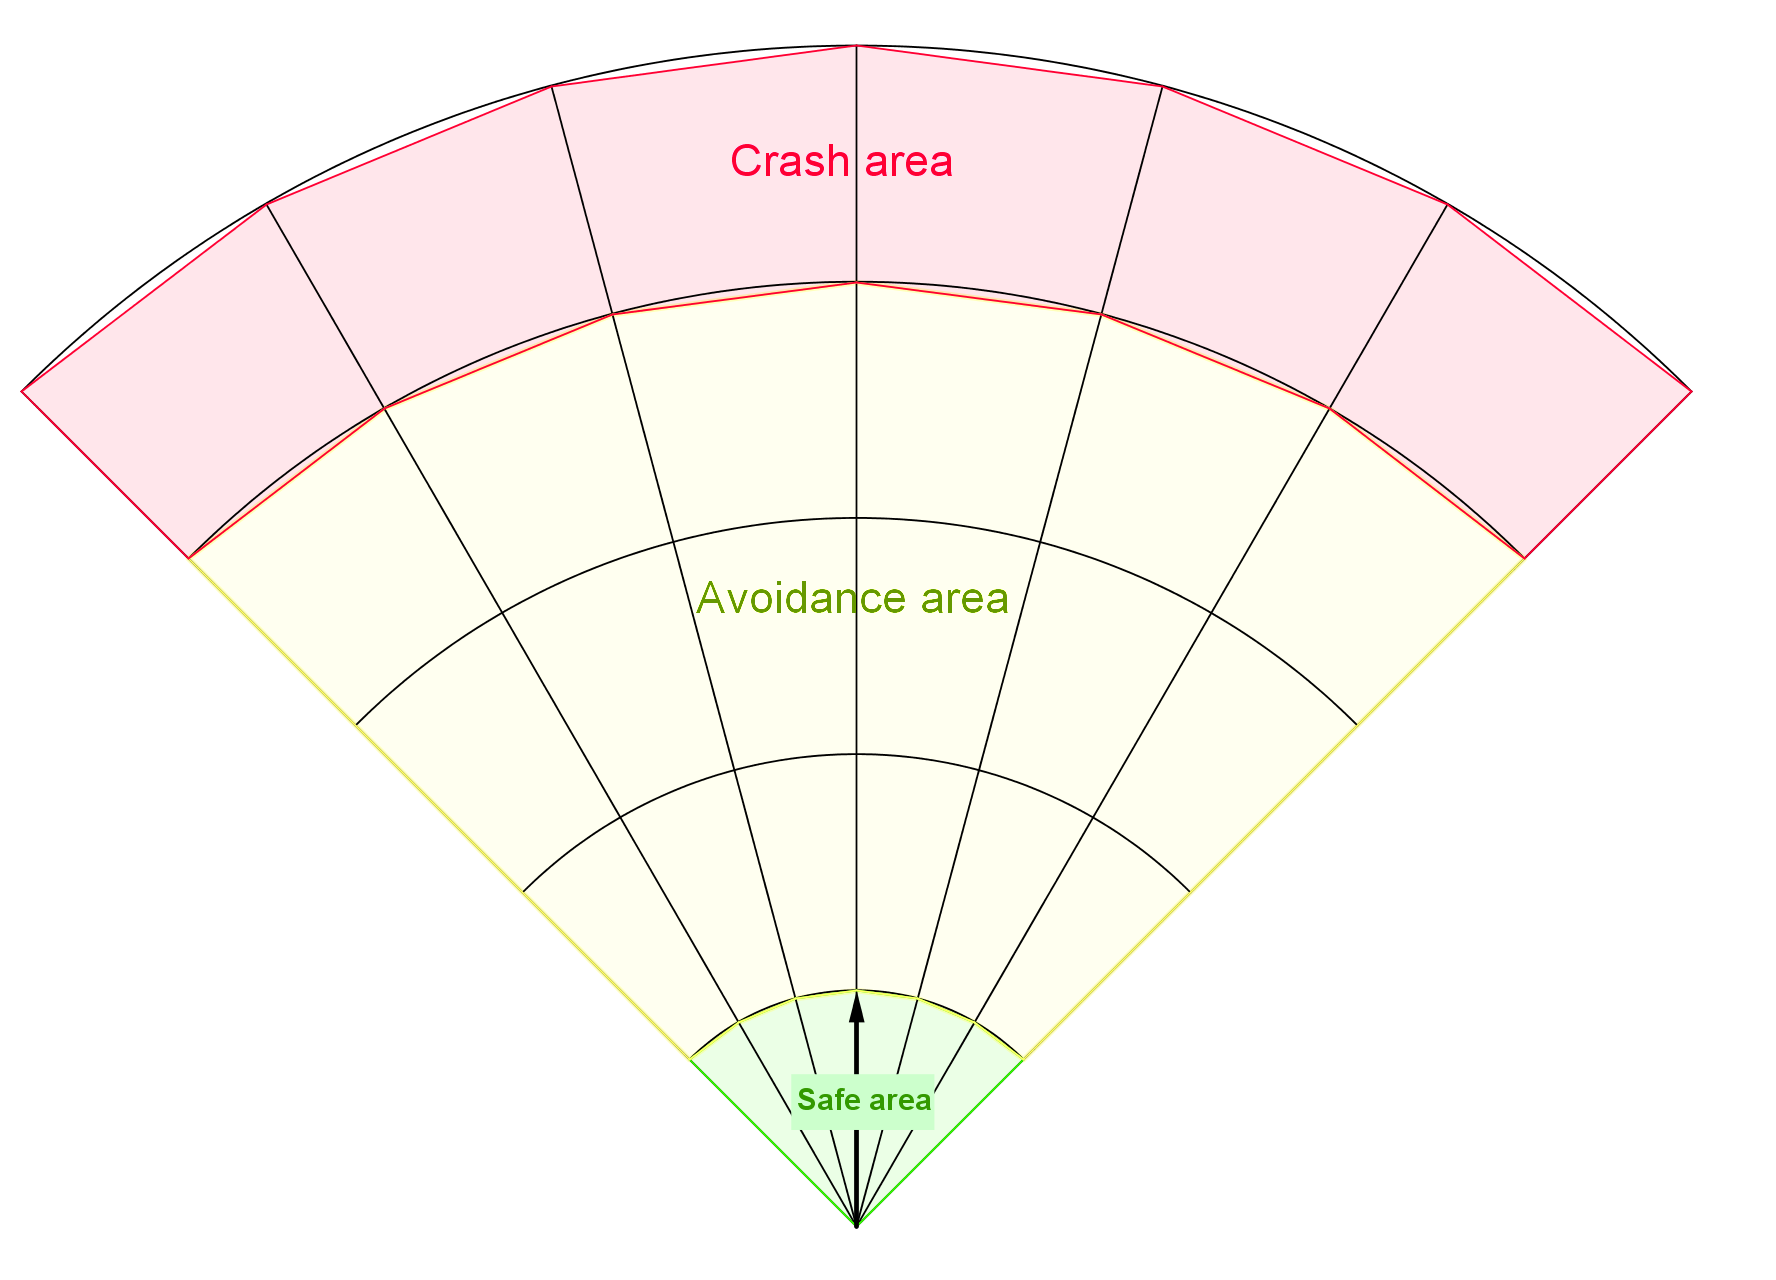
\includegraphics[width=0.9\linewidth]{\FIGDIR/08FieldOfViewZones.png} 
    \caption{Field of view zones}
    \label{fig:FieldOfViewZones}
    \end{subfigure}
    \begin{subfigure}{0.5\textwidth}
    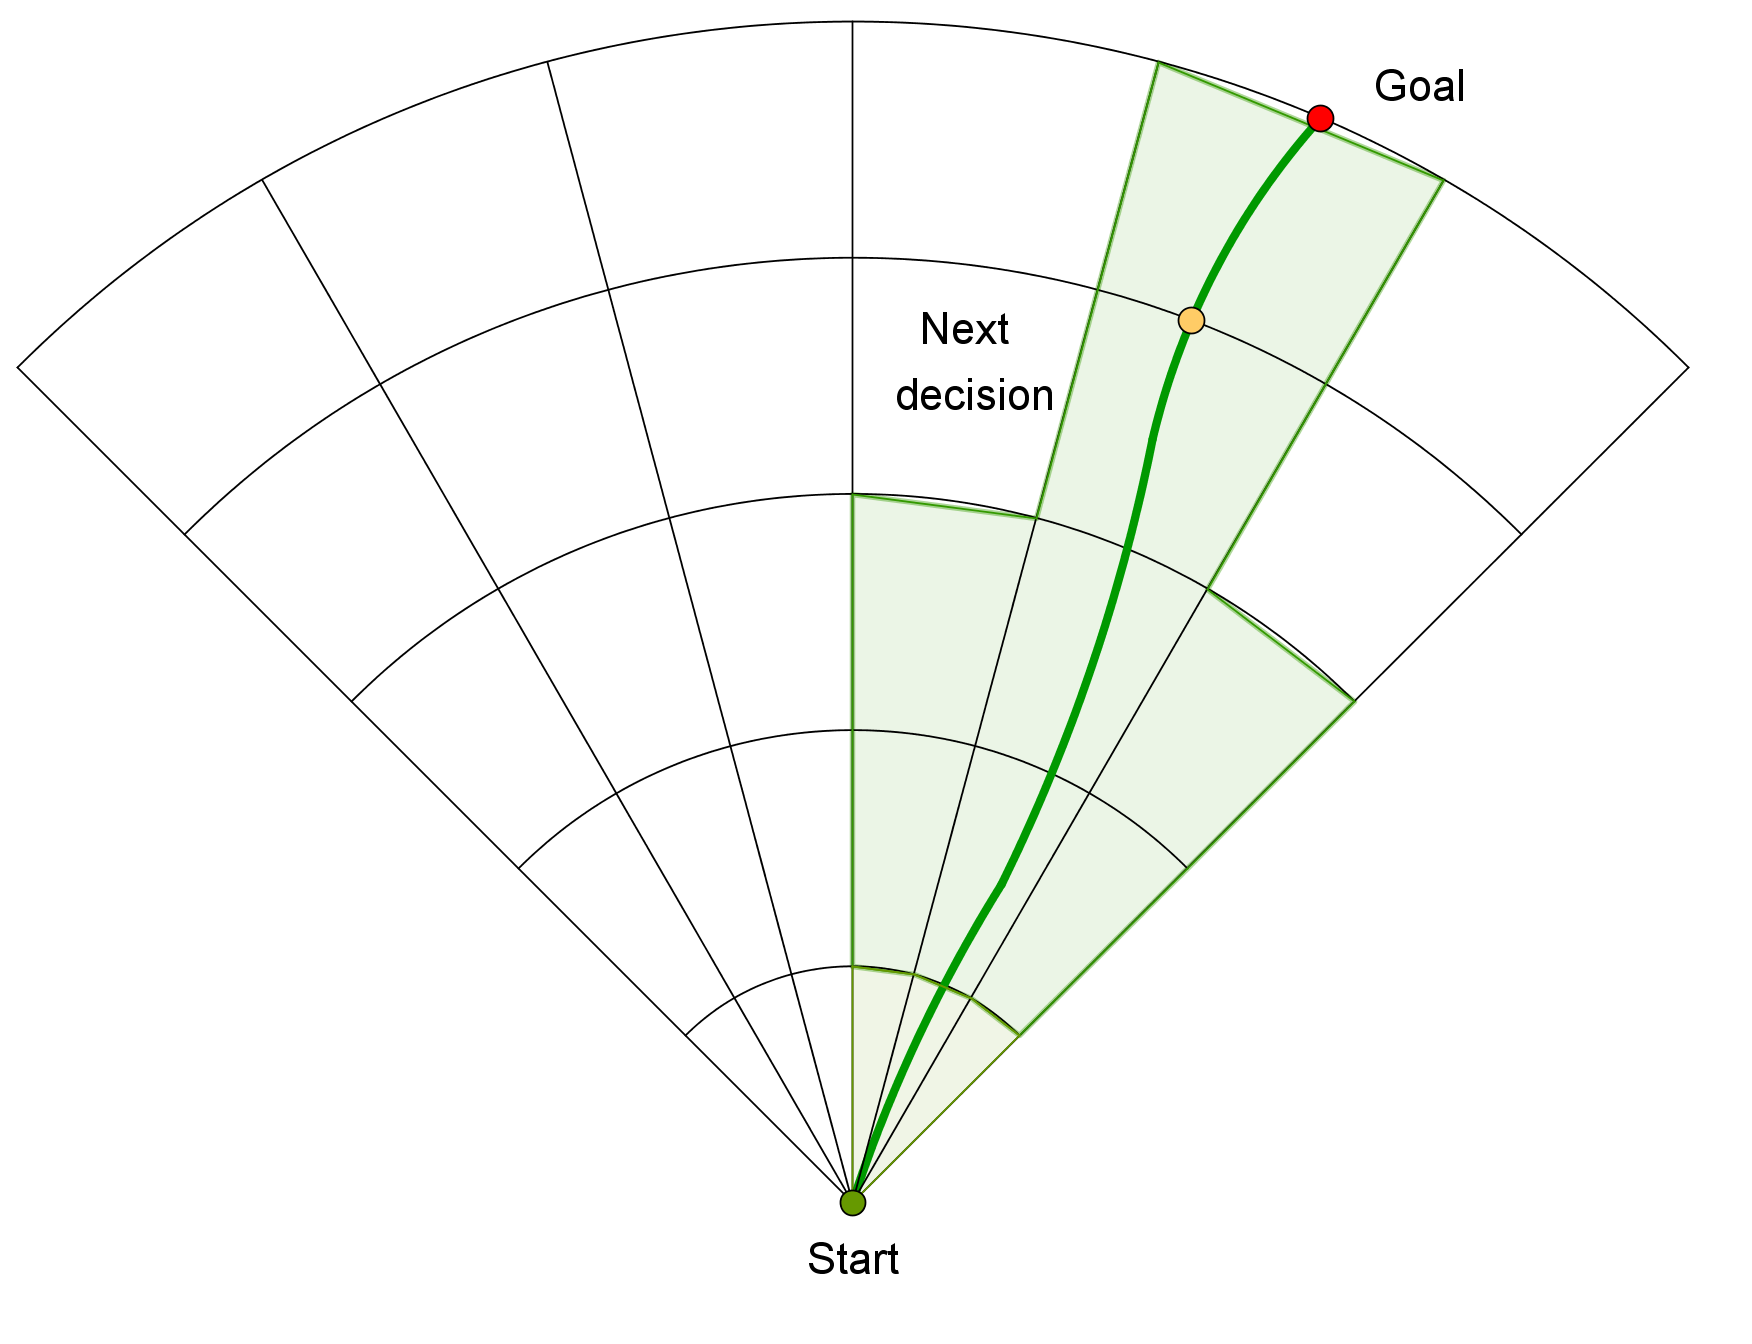
\includegraphics[width=0.9\linewidth]{\FIGDIR/09PathCalculation.png}
    \caption{Avoidance path}
    \label{fig:PathCalculation}
    \end{subfigure}
    
\caption{Determination of avoidance path}
\label{fig:Avoidance}
\end{figure}

Moreless the avoidance strategy for unicycle with defined control strategy $\Omega$ and voting algorithm $\gamma$ is presented in (\ref{eq:avoidanceStrategy}). Given control has been simulated in (\ref{s:simulationruns}) with conservative approach (\ref{s:conservativeapproach}).
